\documentclass[11pt,spanish]{article}

\usepackage{listings}             
\usepackage{anysize} 
\usepackage{graphicx}
\usepackage[spanish]{babel}
\usepackage[utf8]{inputenc}
\usepackage{xcolor}
\usepackage{wrapfig}


\renewcommand\lstlistingname{Código}
\lstset{language=Python}
\marginsize{1cm}{1cm}{2cm}{2cm}
\selectlanguage{spanish}
\lstset{
language=Python,
 backgroundcolor=\color{red!75!green!50!blue!25},
 frame=single,
literate=
  {á}{{\'a}}1 {é}{{\'e}}1 {í}{{\'i}}1 {ó}{{\'o}}1 {ú}{{\'u}}1
  {Á}{{\'A}}1 {É}{{\'E}}1 {Í}{{\'I}}1 {Ó}{{\'O}}1 {Ú}{{\'U}}1
  {à}{{\`a}}1 {è}{{\`e}}1 {ì}{{\`i}}1 {ò}{{\`o}}1 {ù}{{\`u}}1
  {À}{{\`A}}1 {È}{{\'E}}1 {Ì}{{\`I}}1 {Ò}{{\`O}}1 {Ù}{{\`U}}1
  {ä}{{\"a}}1 {ë}{{\"e}}1 {ï}{{\"i}}1 {ö}{{\"o}}1 {ü}{{\"u}}1
  {Ä}{{\"A}}1 {Ë}{{\"E}}1 {Ï}{{\"I}}1 {Ö}{{\"O}}1 {Ü}{{\"U}}1
  {â}{{\^a}}1 {ê}{{\^e}}1 {î}{{\^i}}1 {ô}{{\^o}}1 {û}{{\^u}}1
  {Â}{{\^A}}1 {Ê}{{\^E}}1 {Î}{{\^I}}1 {Ô}{{\^O}}1 {Û}{{\^U}}1
  {œ}{{\oe}}1 {Œ}{{\OE}}1 {æ}{{\ae}}1 {Æ}{{\AE}}1 {ß}{{\ss}}1
  {ű}{{\H{u}}}1 {Ű}{{\H{U}}}1 {ő}{{\H{o}}}1 {Ő}{{\H{O}}}1
  {ç}{{\c c}}1 {Ç}{{\c C}}1 {ø}{{\o}}1 {å}{{\r a}}1 {Å}{{\r A}}1
  {€}{{\EUR}}1 {£}{{\pounds}}1
}


\title{\vspace{-3cm}\begin{flushleft}\textbf{Actividad 9}\end{flushleft}}
\author{\hspace{-9.6cm}\textsc{Andrés Ignacio Rodríguez Mendoza}}
\date{}

\begin{document}

\begin{wrapfigure}{r}{0.2\textwidth}
  \begin{center}
   \vspace{-5.4cm} 
\includegraphics[width=0.15\textwidth]{uni}
  \end{center}
\end{wrapfigure}

\maketitle  
\begin{center}
\rule{\textwidth}{1pt}
\end{center}

$$\alpha$$

\section*{Código}

\begin{lstlisting}[caption=Código para calcular errores]

import numpy as np
from scipy import integrate
import matplotlib.pyplot as plt
import math

t=100
n=6
# Arreglos 
x=[]
TT0_0=[]
TT0=[]
x_0=np.linspace(0.001,np.pi + 0.001, t)

#   el integrando
I = lambda x,a: 1/np.sqrt(np.cos(x) - np.cos(a))

#   Calcular los valores reales
for i in range(t):
#   la integral
    theta_0=x_0[i]
    T_0 , err= integrate.quad(I, 0, theta_0, args=(theta_0,))
    
    
#   el periodo
    TT0_0.append((4/np.sqrt(2)) * T_0)

    
#   Ciclo para cada gráfica:    
for v in range(n):
    
#   lista de los valores de error    
    err=[]
        
    for i in range(t):
    
    
        theta_0 = x_0[i]
        T0=1

#   la sumatoria        
        for u in range(v):
            
            T0 += math.pow( math.factorial(2*(u+1)) / (math.pow( math.pow(2,(u+1)) * math.factorial(u+1) , 2 ) ) , 2 ) * math.pow( np.sin(theta_0 / 2), 2*(u+1) )   
            
#   los valores en la lista de errores           
        err.append(100*(np.absolute(2 * np.pi * T0 - TT0_0[i])/TT0_0[i]))
   
#   Gráfica, cada aproximación    
    plt.plot(x_0 * 180 / np.pi, err, '-.', linewidth=2, label='$T %i $' % (2*v))
    
    

   
#   Gráfica desviación
plt.title('Errores relativos de las series de potencias')
plt.xlabel(r'$ \theta _0 (deg)$')
plt.ylabel("Error Relativo (%)")
plt.xlim(0,120)
plt.ylim(0,1)
plt.xticks(np.arange(0,130,10))
plt.yticks(np.arange(0,1.1,0.1))
plt.legend(loc='center left', bbox_to_anchor=(1, 0.5))
plt.grid()
plt.show()

\end{lstlisting}

\begin{lstlisting}[caption=Segmento de código para la serie de Maclaurin]


Err=[]
for i in range(t):
    theta_0 = x_0[i]
    T0=1
    for u in range(80):
        sen=0
# la sumatoria para maclaurin en el seno
        for k in range(50):
            sen += math.pow(-1,k)/math.factorial(2*k+1) * math.pow(theta_0/2, 2*k+1)
            
        T0 += math.pow( math.factorial(2*(u+1)) / (math.pow( math.pow(2,(u+1)) * math.factorial(u+1) , 2 ) ) , 2 ) * math.pow( sen , 2*(u+1) )   
    
    Err.append(100*(np.absolute(2 * np.pi * T0 - TT0_0[i])/TT0_0[i]))

plt.plot(x_0 * 180 / np.pi, Err, '-.',color='k', linewidth=2, label='$T %i $' % (2*v))
plt.title('Error usando serie de Maclaurin')
plt.xlabel(r'$ \theta _0 (deg)$')
plt.ylabel("Error Relativo (%)")
plt.xlim(0,180)
plt.ylim(0,1)
plt.xticks(np.arange(0,190,10))
plt.yticks(np.arange(0,1.1,0.1))
plt.legend(loc='center left', bbox_to_anchor=(1, 0.5))
plt.grid()
plt.show()

\end{lstlisting}

\section*{Gáficas}

\centering

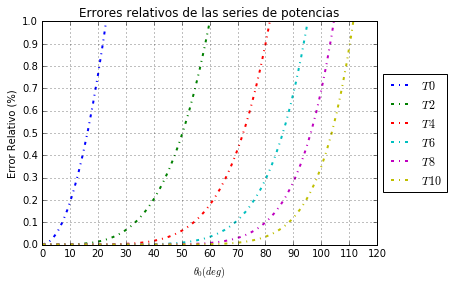
\includegraphics[scale=1]{err}\\
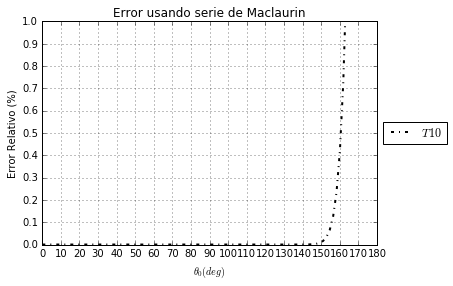
\includegraphics[scale=1]{mac}\\





\end{document}
